\chapter{Prototype}
\label{chap:prototype}

\begin{chapterintro}

In this chapter, we will describe the prototype we developed following the architecture described in the previous chapter.
 
\end{chapterintro}

\cleardoublepage

\section{Overview of the system}

For this system, we developed a prototype utilising the architecture explained in chapter \ref{chap:architecture}. To do so, we deployed the following modules and subsystems:

\begin{enumerate}
 \item A Javascript client, that will connect to the system and act as an user interface.
 \item A Front-end controller, written in python, that will handle the interaction between the different modules-
 \item A chatbot using chatscript, to handle question analysis and chit-chat interaction.
 \item An Apache Solr instance, where all the semantic data will be loaded.
\end{enumerate}

In parallel to all this, both a web scraper using scrapy to recover the relevant data, and an uploader to post the data to Solr.

\subsection{Chat client}
\label{sec:chatclient}

In our prototype, the interaction with the system is done via a web client that provides a chat box and an iframe where the content is located. When the user first opens the page, it's greeted by the bot, and provided with a   short explanation of how the client works.

\begin{figure}[!htbp]
    \centering
    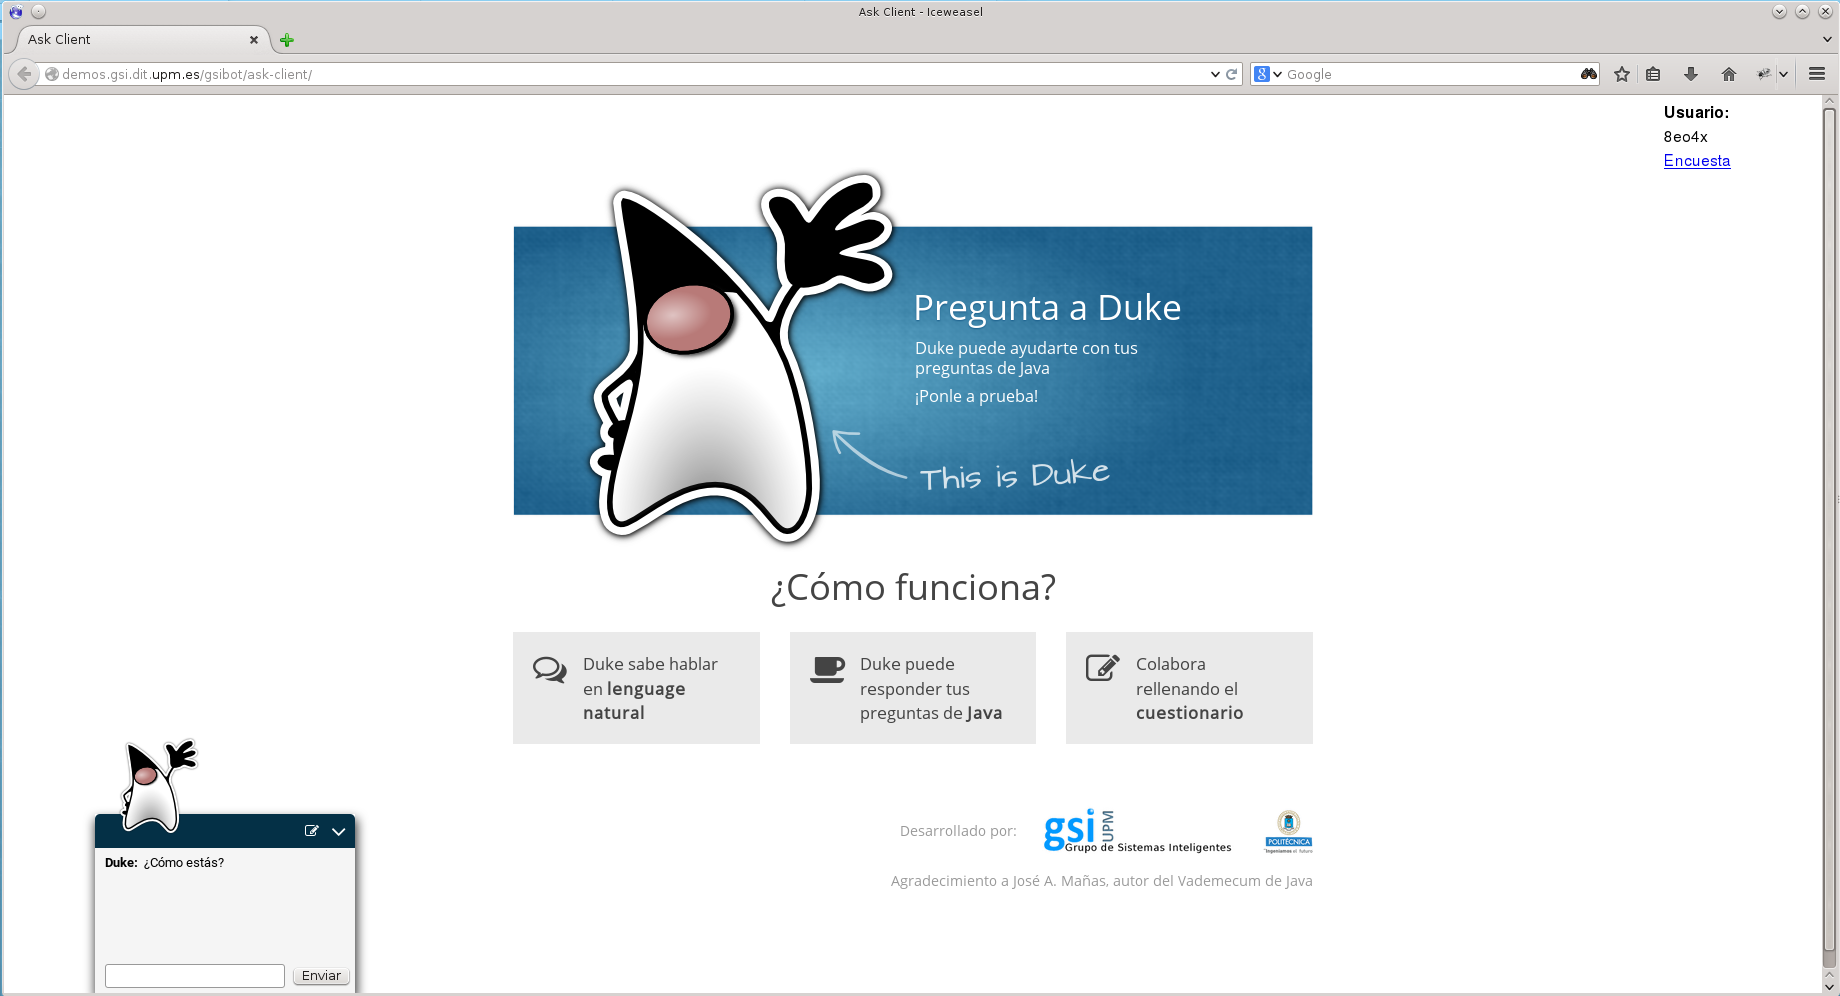
\includegraphics[width=0.7\textwidth]{img/screens/ask-client.png}
    \caption{Web interface for the client.}
    \label{fig:chat1}
\end{figure}

The client is made using web technologies: HTML, CSS and Javascript, and uses Ajax to communicate with the server sending the user questions and handling the response.

\emph{Add example of JSON request}

\lstinputlisting[language=JavaScript, firstline=77, lastline=88]{code/prot/ask.js}

\subsection{Front end controller}

The Front end controller is the main control module in our system. It handles the requests received from the client described in \ref{sec:chatclient}, and proceeds to triggers the required modules, as well as executing the \ac{OoB} commands received from each module. This module is provided as a web service, and therefore we have chosen Flask~\cite{flask0101} and Apache's mod\_wsgi~\cite{modwsgi} to deploy it. In the following subsections we will describe how it works as well as its work-flow structure.

\subsubsection{Functional Model}

The function of this module is returning the answer to the user, formed as JSON, by triggering the appropriate modules and reacting to their responses. To do so, it follows a process explained in the UML diagram shown in Figure \ref{fig:fe-model1}.

\begin{figure}[!htbp]
    \centering
    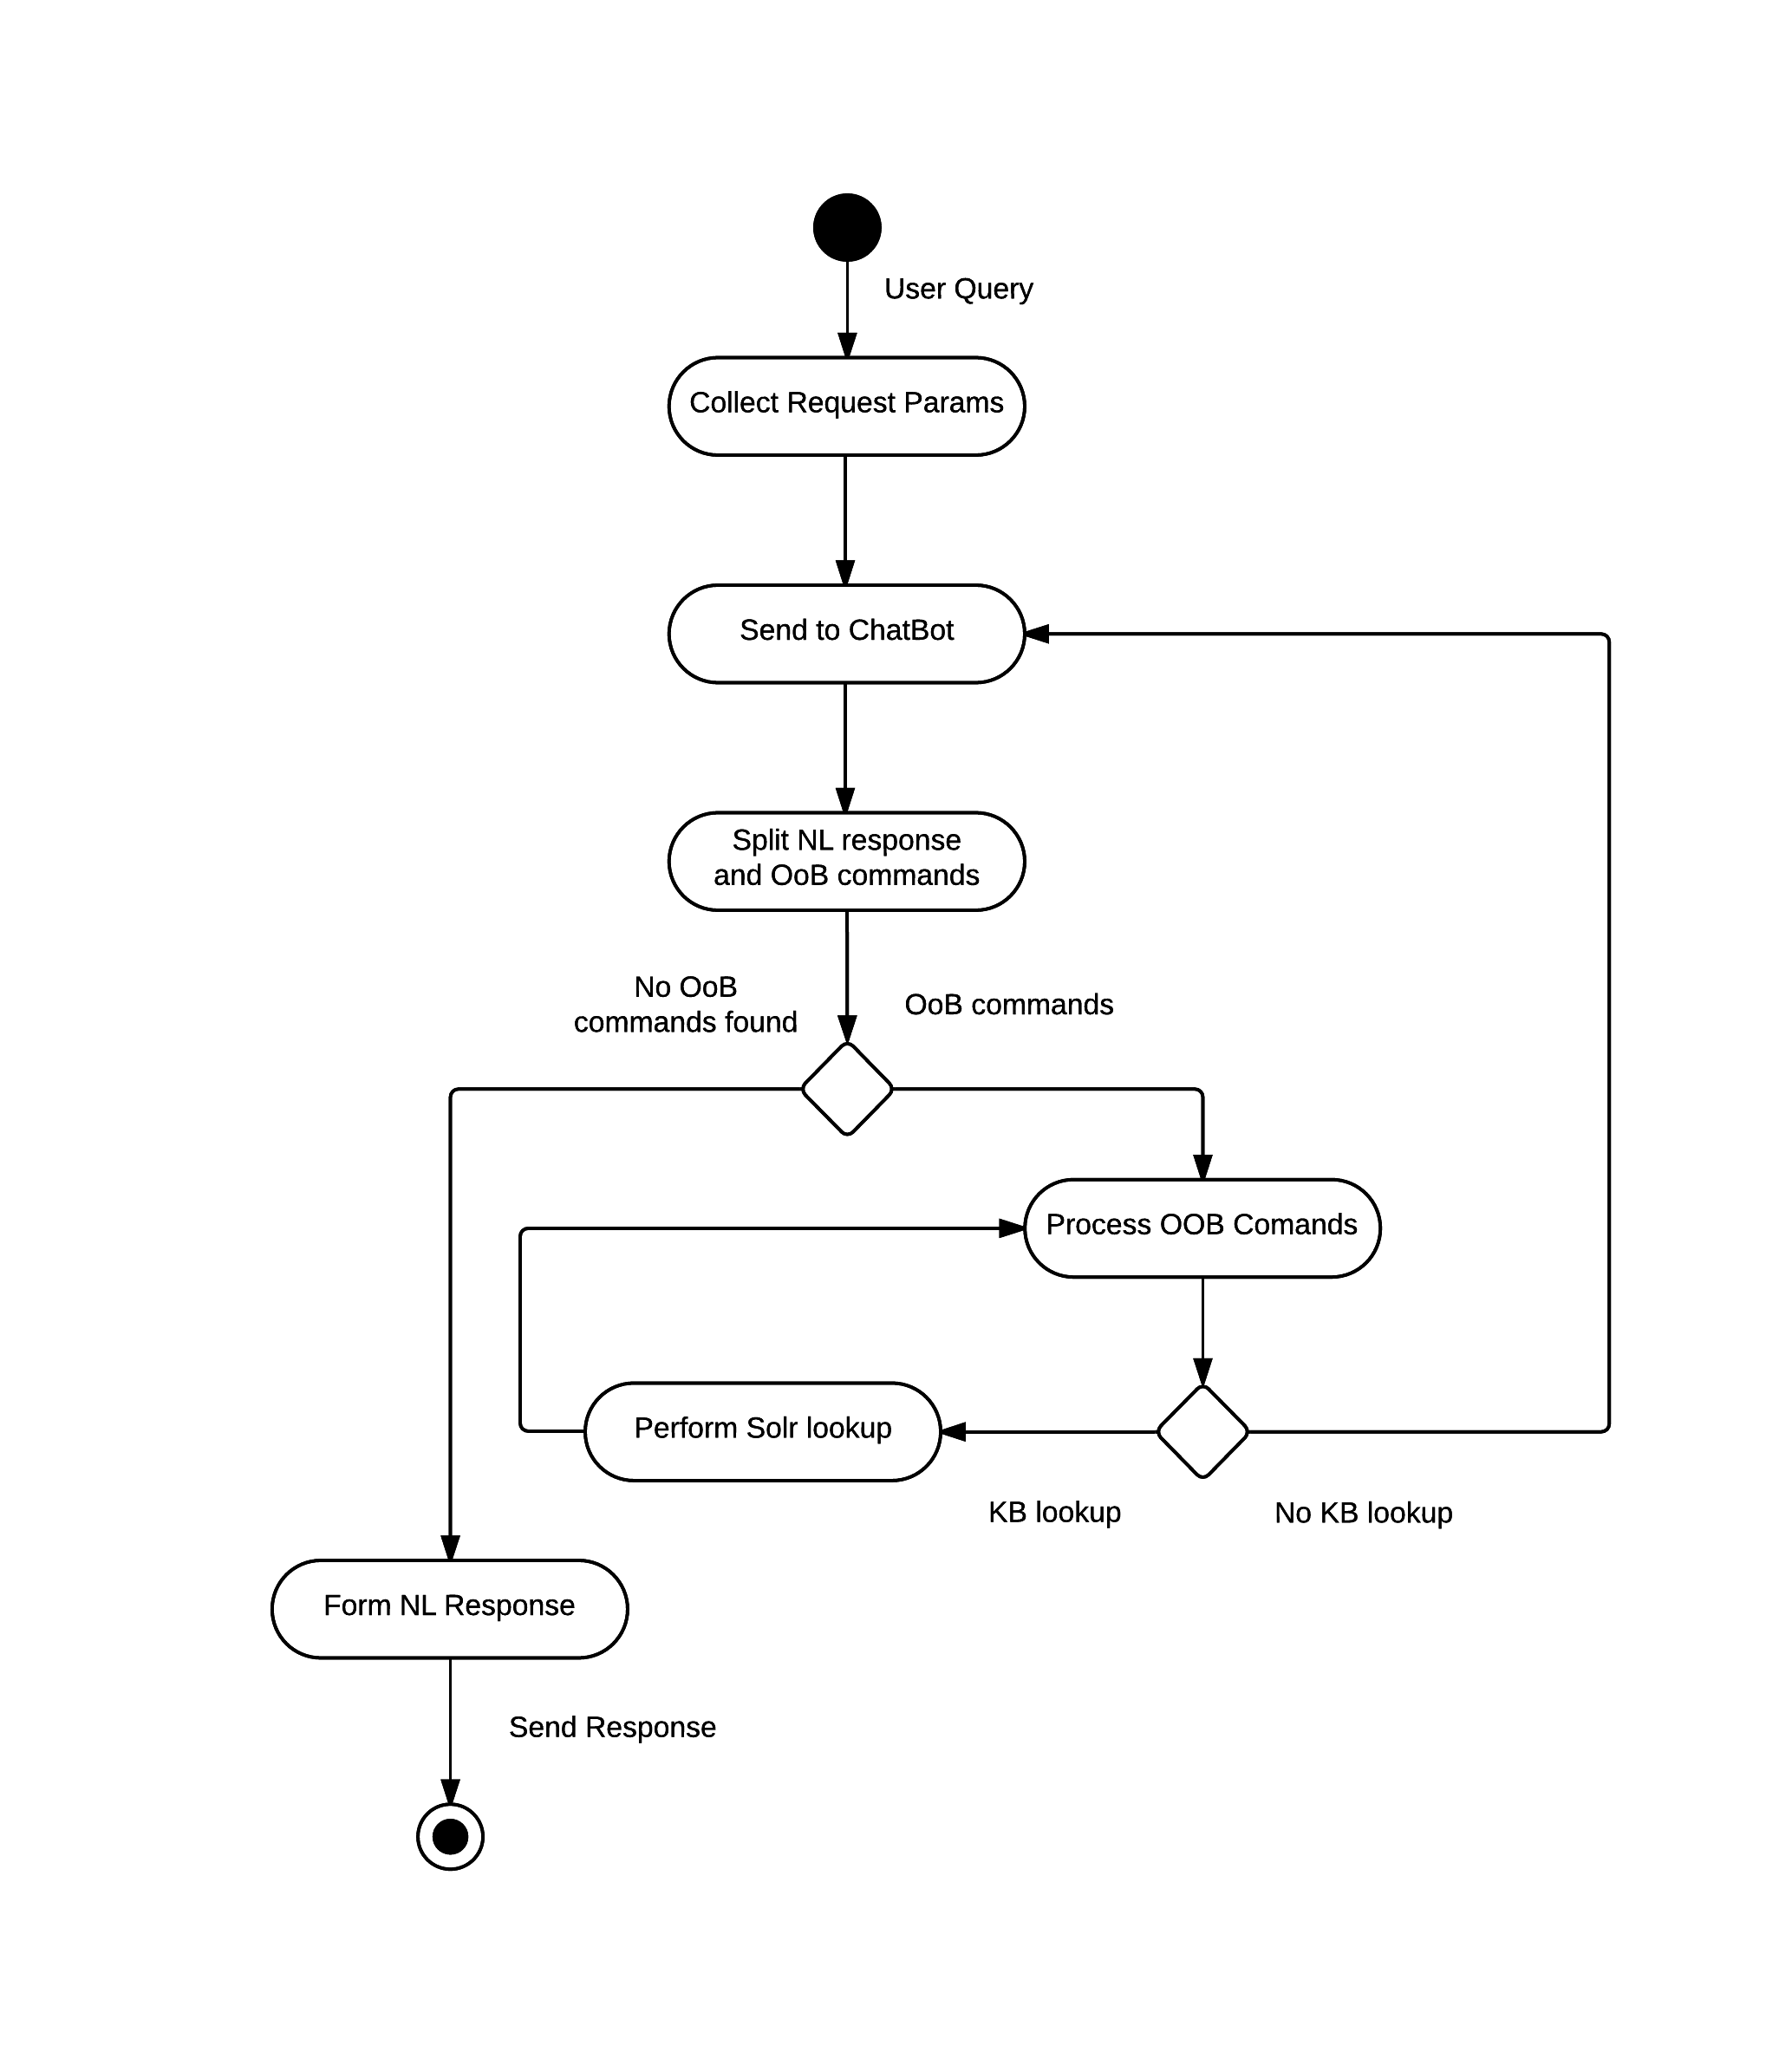
\includegraphics[width=0.6\textwidth]{img/prot/activityDiagram.png} 
    \caption{UML diagram of the process followed by the controller.}
    \label{fig:fe-model1}
\end{figure}

\begin{itemize}
 \item \textbf{Request parsing:} The client sends the query as JSON using a HTTP request to the front-end controller. This JSON is recovered and processed into a python dictionary.
 \item \textbf{Send to ChatBot:} The user query is sent to the ChatBot so it's processes and a response, either \ac{NL} or \ac{OoB}, is generated.
 \item \textbf{Split \ac{NL} response and \ac{OoB} commands} The response in the previous step is split in \ac{NL} and {OoB} commands, to process each one appropriately.
 \item \textbf{\ac{OoB} command processing:} Read the \ac{OoB} commands and take the appropriate steps for each one of them.
 \item \textbf{Solr Lookup:} If a lookup in the Knowledge base is required, send the query to Solr.
 \item \textbf{Form Response:} Once there are no more \ac{OoB} commands, form the actual response in JSON and send it to the user.
\end{itemize}

% Add the workflow of the controller.

\subsubsection{Structural Model}

In this section we will describe the structure followed designing the front end controller. In figure \ref{fig:fe-methods1} we show the method structure of the controller.
\begin{figure}[!htbp]
    \centering
    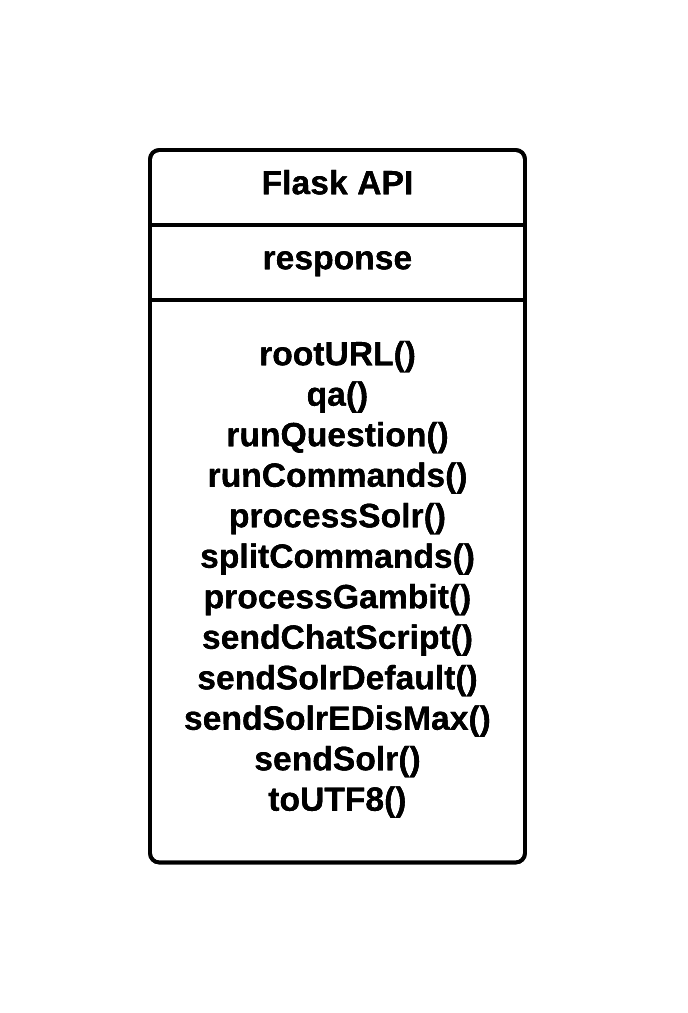
\includegraphics[width=0.4\textwidth]{img/prot/controllerStructure.png}
    \caption{Front end controller structure}
    \label{fig:fe-methods1}
\end{figure}

Now we will proceed to describe each of the methods shown in the figure.

\begin{itemize}
  \item \textbf{rootURL()} will be triggered whenever the base URL for the controller is requested. It will act in the same way than the qa() method.
  \item \textbf{qa()} this function will recover the request parameters, shown in table \ref{tab:fe-qparams}, and start the process to understand the user query, in order to return the appropriate response, whose parameters are shown on table \ref{tab:fe-rparams}.
  \item \textbf{runQuestion()} in this function, we will simply run the question once throught ChatScript, and then start the main command processing.
  \item \textbf{runCommands()} Given the \ac{NL} response from ChatScript, it will split the \ac{OoB} commands and start processing each one of them, as well as their responses, adding commands to the queue as needed.
  \item \textbf{processSolr()} For the solr command, this method will construct the solr query, and keep sending it to Solr increasing its fuzziness level, until an answer is found, or a maximum fuzziness is reached, in which case it will return the empty solr response.
  \item \textbf{splitCommands()} Taking a \ac{NL} sentence as a parameter, this method will return both a list with all the \ac{OoB} commands in the sentence, as well as the \ac{NL} part of the sentence, or an empty string if the sentence was made only of \ac{OoB} commands. 
  \item \textbf{processGambit()} when a direct search does not return any answer, the system will perform a broader search in Solr. This is further explained in section \ref{sec:solr}.
  \item \textbf{sendChatScript()} This function will process the interaction with ChatScript, both sending the questions and handling the responses. For more details, see section \ref{sec:chatbot}.
  \item \textbf{sendSolrDefault()} Given a question and no other parameters or information, this function will send said question to Solr, so it will go through the default processing. This is mainly unused.
  \item \textbf{sendSolrEDisMax()} When a gambit is needed, send the question to Solr using an eDisMax query, which will search in different fields, valuing each field using a given weight. 
  \item \textbf{sendSolr()} Used by the rest of the Solr related methods, this function will handle sending the payload given as parameter to Solr, and returning the JSON response.
\end{itemize}

% TODO: change for tables
\begin{center}
  \begin{table}
    \begin{tabular*}{0.7\textwidth}{@{\extracolsep{\fill}} | c | c | p{0.5\textwidth} |}
      \hhline{|-|-|-|}
      \textbf{Parameter} & \textbf{Name} & \textbf{Description} \\ \hhline{|=|=|=|}
      question & User's question & The question submitted by the user. \\ \hhline{|-|-|-|}
      bot & Bot & The bot the query will be send to. \\ \hhline{|-|-|-|}
      username & The user & A random identifier for the user communicating with the bot. \\ \hhline{|-|-|-|}
      \end{tabular*}
    \caption{Parameters in the query received by the front end controller.}
    \label{tab:fe-qparams}
  \end{table}
\end{center}

\begin{center}
  \begin{table}
    \begin{tabular*}{0.7\textwidth}{@{\extracolsep{\fill}} | c | c | p{0.5\textwidth} |}
      \hhline{|-|-|-|}
      \textbf{Parameter} & \textbf{Name} & \textbf{Description} \\ \hhline{|=|=|=|}
      Answer & The Bot's response & The \ac{NL} response generated by the bot. \\ \hhline{|-|-|-|}
      Resource & An URL & The url of the relevant document where the information is, if existent. \\ \hhline{|-|-|-|}
      \end{tabular*}
    \caption{Parameters in the query sent back to the client.}
    \label{tab:fe-rparams}
  \end{table}
\end{center}

Finally, we will describe the \ac{OoB} commands that the system will be able to process.

\begin{itemize}
 \item \textbf{¬sendSolr} this command is issued whenever a question matches the pattern specified to request information about a Java topic.
 \item \textbf{¬solrResponse} after a search is performed in Solr, this command is issued to indicate whether or not a response has been found, and returning said response.
 \item \textbf{¬solrLinks} a special Solr search, looking for related topics in Solr.
 \item \textbf{¬solrLinksResponse} as a response to the solrLinks command, returns a list with the related topics.
 \item \textbf{¬gambit} perform an eDisMax search in Solr, using the full user question.
 \item \textbf{¬gambitResponse} returns the title of the most relevant document found in the eDisMax search.
 \item \textbf{¬gambitUnknown} issued when no document with a high enough score is found in Solr.
 \item \textbf{¬resource} sets the url to be displayed in the final response returned to the client.
 \item \textbf{¬label} sets the title of the found document as the label for the response.
\end{itemize}

The syntaxes of the commands is specified in table \ref{tab:oob-commands}.
\begin{center}
  \centering
  \begin{table}
    \begin{tabular*}{0.7\textwidth}{@{\extracolsep{\fill}} | c | c | p{0.35\textwidth} |}
      \hhline{|-|-|-|}
      \textbf{Command} & \textbf{Syntaxes} & \textbf{Description} \\ \hhline{|=|=|=|}
      ¬sendSolr & ¬sendSolr \textit{reqfield} \textit{doctitle} & Searchs in solr for the \textit{doctitle} and returns the \textit{reqfield} field.  \\ \hhline{|-|-|-|}
      \multirow{2}{*}{¬solrResponse} & ¬solrResponse \textit{unknown} & The requested document was not found in Solr. \\ \cline{2-3}
				     & ¬solrResponse \textit{reqfield} \textit{response} & Returns as \textit{response} the data of the field \textit{reqfield}. \\ \hhline{|-|-|-|}
      ¬solrLinks & ¬solrLinks \textit{linklist} & Asks for a search in Solr for the name of the topics given as an uri in the linklist \\ \hhline{|-|-|-|}
      ¬solrLinksResponse & ¬solrLinksResponse \textit{nameslist} & Sets the response for the ¬solrLinks command, returning the first name of the links. \\ \hhline{|-|-|-|}
      ¬gambit & ¬gambit \textit{topic}& Asks for a eDisMax search on Solr, passing the full question. \\ \hhline{|-|-|-|}
      ¬gambitResponse & ¬gambitResponse \textit{gambittopic} & After performing an eDisMax search, returns \textit{gambittopic} as the suggested topic. \\ \hhline{|-|-|-|}
      ¬gambitUnknown & ¬gambitUnknown & After performing an eDisMax search, indicates that no relevant document has been found. \\ \hhline{|-|-|-|}
      ¬resource & ¬resource \textit{URL} & Sets \textit{URL} as the resource to be displayed in the client \\ \hhline{|-|-|-|}
      ¬label & ¬label \textit{topic} & Sets \textit{topic} as the concept of the response \\ \hhline{|-|-|-|}
      \end{tabular*}
    \caption{Parameters in the query sent back to the client.}
    \label{tab:oob-commands}
  \end{table}
\end{center}

\subsection{ChatBot}
\label{sec:chatbot}

The ChatBot handles the processing of the natural language input from the user, and controls the conversation. To do so, it uses the chat engine ChatScript, described in section \ref{subsec:chatscript}.

\subsubsection{The rules}

\subsubsection{Using spanish dictionaries}

% Explain how chatscript works.

\subsection{Solr instance}
\label{sec:solr}

% Solr - add the relevant schema portions and how they work.

\section{Use cases}

% ¿? Something something... or something else?